\documentclass[journal]{IEEEtran}
\usepackage{graphicx}
\usepackage[scriptsize]{caption}
\renewcommand{\arraystretch}{1.1}

\begin{document}

\newcommand{\labtitlegen}{
    \twocolumn[{
    \begin{center}
        \LARGE\labtitle \\ \bigskip \large\name \\ \bigskip
        \labsection \\ 
        \textbf{TA} \\ \taname \\ \bigskip \textbf{Lab Partners} \\
        \partnername
    \end{center}
    }]
}

%% Change these variables
\newcommand{\labtitle}{Experiment 2: DC and AC Circuits}
\newcommand{\name}{Vladimir Vysotsky}
\newcommand{\labsection}{Section 2, Wednesday 8AM}
\newcommand{\labdate}{January 28, 2015}
\newcommand{\taname}{Elwin Martin}
\newcommand{\partnername}{Kari Kawashima, Merrick Campbell}


%% This creates your lab cover page.
\labtitlegen

\newcommand{\mval}[3]{$#1 \pm #2 #3$}



\section{Introduction}
Circuit analysis is based on several key assumptions about how certain circuit
elements behave, in terms of resistance, capacitance, and a few other
properties. We seek to justify a few of these assumptions. For DC circuits, one
of the primary assumptions is the linearity of resistance - current through a
resistor is directly proportional to voltage. A diode behaves much less
linearly, but follows an exponential curve when the voltage is much larger than
0. An RC circuit follows an exponential curve getting closer to the target
voltage (whatever is being applied across its branch of the circuit). An RLC
circuit, when driven, displays a resonance peak, which can be calculated from
the values of the inductor and capacitor (the reactive circuit elements).

These assumptions will be tested by measuring these circuit elements and
comparing the predictions, sometimes indirectly, to accepted or otherwise
measured values.

\section{Results}

We used a signal generator to create variable waveforms that allow us to
quickly measure how the resistance of a particular circuit element changes
under varying voltage.

\begin{figure}[ht!]
\centering
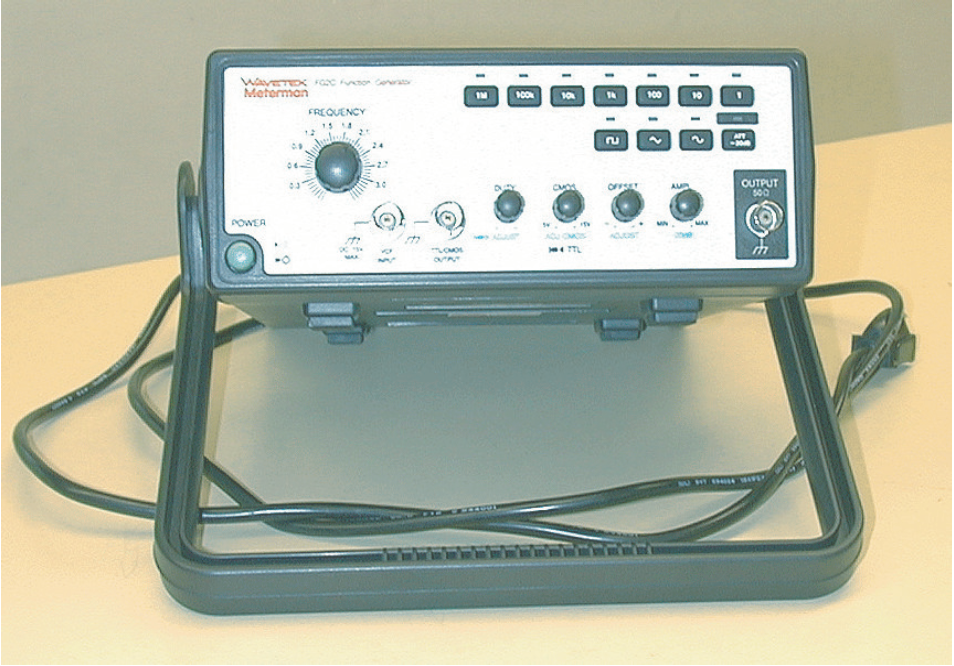
\includegraphics[width=40mm]{signal_gen.png}
\caption{Variable signal generator.}
\label{fig:sig_gen}
\end{figure}

The signals are accessed via a breakout board which connects to the output of
the signal generator. It is shows in Figure~\ref{fig:breakout}. It allows access to both
outputs of the generator simultaneously.

For the remainder of these experiments, a resistor will be used to calculate
the current through its branch of the circuit (this will be used to create IV
curves for unknown circuit elements, by measuring the voltage across the
element and the current through the resistor). It has a resistance of
\mval{98.7}{0.05}{\Omega}, and will be referred to as r.

\begin{figure}[ht!]
\centering
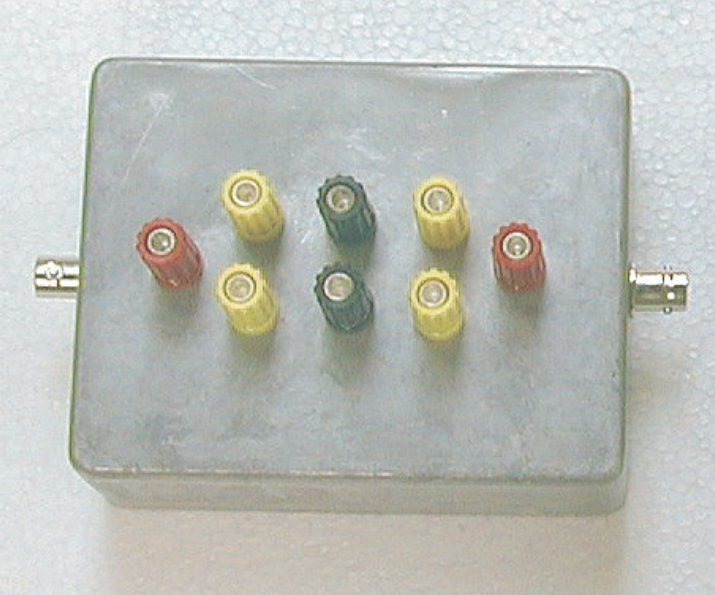
\includegraphics[width=40mm]{breakout.png}
\caption{Signal generator breakout board.}
\label{fig:breakout}
\end{figure}

The first test performed was on a parallel pair of resistors. One is the
aforementioned resistor r, and the other is a larger resistor R, measured by a
multimeter to be \mval{993}{0.5}{\Omega}. The current through resistor r is
calculated using the relation I = V/R and plotted against the voltage measured
across resistor R. The circuit was driven by a triangular wave at approximately
10 Hz from the signal generator. Data was collected at 5,000 samples per second
for 1,000 points, making the sample approximately two whole periods. The data
    is presented in Figure~\ref{fig:res_series}.

\begin{figure}[ht!]
\centering
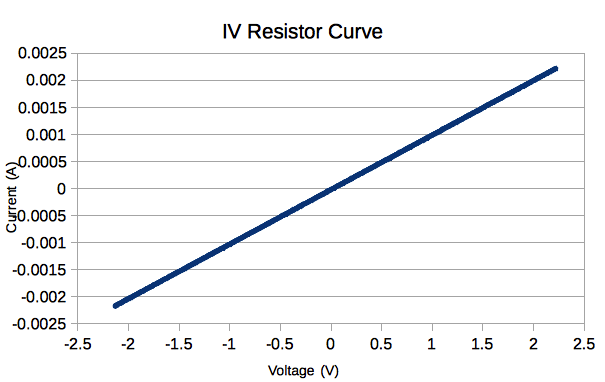
\includegraphics[width=70mm]{iv_resistor.png}
\caption{The IV curve for a resistor, being driven by a triangle wave.}
\label{fig:res_series}
\end{figure}

The resistor R was then replaced with a diode, oriented so that the diode
allowed a current through it when the voltage measured across it was positive.
Diodes should, unlike resistors, exhibit non-linear voltage response, which
should be visible in Figure~\ref{fig:dio_series}. The remainder of the setup
was kept the same.

\begin{figure}[ht!]
\centering
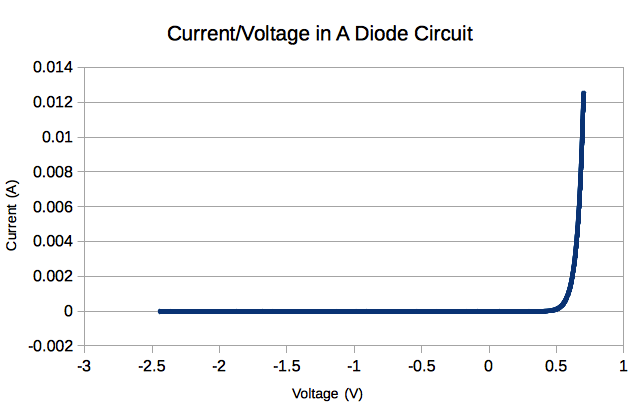
\includegraphics[width=70mm]{iv_diode.png}
\caption{The IV curve for a diode, being driven by a triangle wave.}
\label{fig:dio_series}
\end{figure}

The diode response curve has a much more interesting, non-linear shape. It
appears to follow an exponential of some sort, though that breaks down at
negative voltages. When driven in the wrong direction, the current through the
diode quickly approaches a constant value $I _0$. That value for this diode in
particular is approximately \mval{2.33}{0.001}{mA}. When driven in the correct
direction, the diode does in fact respond as an exponential - more
specifically, the IV curve can be theoretically described by
Equation~\ref{diode_iv}.

\begin{equation}
\label{diode_iv}
I + I_0 = I_0 \left( e^{\frac{|e|V}{n k_B T}} \right)
\end{equation}

This accounts for the shape of the diode's IV curve.

A similar wiring is used in the analysis of AC circuits, except the voltage is
measured across the entire circuit and across a single circuit element, rather
than across each element individually.

A resistor at \mval{119.5}{0.05}{k \Omega} was placed in series with a $1.0 \mu
F$ capacitor. The uncertainty on the capacitance is not known, so while these
measurements will have a regression analysis performed on it to find a
statistical uncertainty, there may be an unknown systematic uncertainty from
the exact value of the capacitor. The signal generator was set to a very low
frequency - 0.4 Hz - so that the capacitor is allowed to charge almost fully
in a single half-period. This allows accurate measurement of the exponential
curve that it follows as it is charging. This response is demonstrated in
Figure~\ref{fig:rc_response}.

\begin{figure}[ht!]
\centering
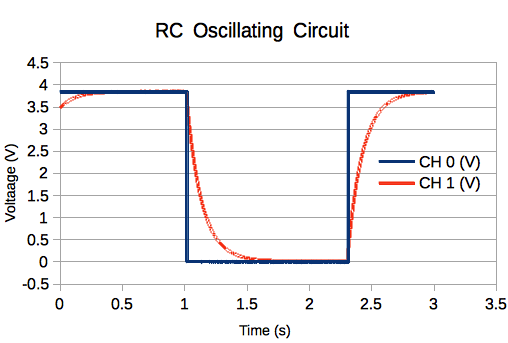
\includegraphics[width=70mm]{rc_response.png}
\caption{Capacitor being charged and discharged under low-frequency square wave.}
\label{fig:rc_response}
\end{figure}

The measurement of RLC circuit response is different from the previous setup.
Instead of being driven by the signal generator, it is connected to the DAQ and
driven by it, with the response being simultaneously measured across a
resistor. This allows accurate measurement of the phase angle and amplitude
response of the RLC circuit under various driving frequencies.

The resistor in this case is \mval{1.00}{0.005}{k \Omega}, the capacitor is $1
\mu F$, and the inductor is 100 mH. The amplitude-response curve is presented in
Figure~\ref{fig:rlc_response}.

\begin{figure}[ht!]
\centering
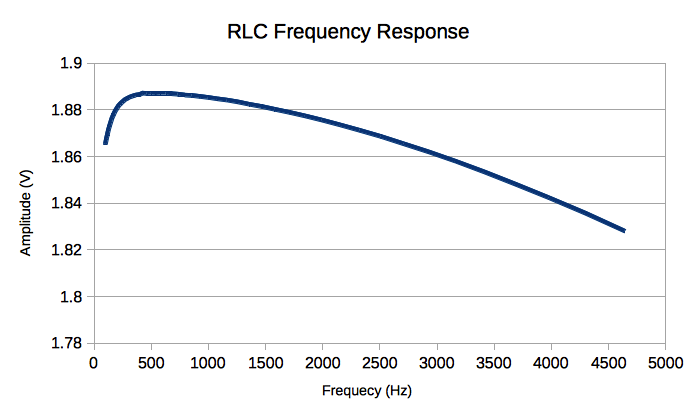
\includegraphics[width=70mm]{rlc_response.png}
\caption{Amplitude response of RLC circuit being driven at various frequencies.}
\label{fig:rlc_response}
\end{figure}

\section{Analysis}

The data in Figure~\ref{fig:res_series} follows a linear curve, and following Ohm's law
\begin{displaymath}
I = \frac{V}{R}
\end{displaymath} 
The slope is the inverse resistance. Performing a linear regression in a
spreadsheet software yields a slope of m = \mval{0.001008}{5E-7}{}. Since the
resistance is the inverse of this, the uncertainty in resistance is 
\begin{displaymath}
\sigma _{\bar R} = \sqrt{\left( \frac{\partial}{\partial m} \frac{1}{m}
\right)^2 \sigma _{\bar m}^2} = \frac{\sigma _{\bar m}}{\bar m^2}
\end{displaymath} 
Which yields a resistance of R = \mval{992.2}{0.5}{\Omega}. This almost exactly
matches the multimeter value of \mval{993}{0.5}{\Omega}, with a difference of
only 0.08\%.

The diode curve in Figure~\ref{fig:dio_series}, though a full description of
how the diode behaves, cannot be used in its entirety to find the constants
describing the diode. In particular, the response curve described by
Equation~\ref{diode_iv} is only followed at positive voltages, and does not
work close to zero. In the interest of extracting the information, the voltages
were thresholded at 0.001 V - everything lower was not included in the
analysis. This had two motivations - it allows an approximation to simplify the
math (presented next), and it was the best-fit region for an exponential.

In addition, some extra process was done to the data - the logarithm of both
sides of the data were taken, giving the following relationship

\begin{displaymath}
ln(I + I_0) = ln(I_0) + \left( \frac{|e|V}{n k_B T} \right)
\end{displaymath}

Because $I_0$ is \mval{2.33}{0.001}{mA}, which is three orders of magnitude
below the threshold for I, it can be ignored in comparison to I, yielding the
following approximation.

\begin{equation}
\label{diode_iv_ln}
ln(I) = ln(I_0) + \left( \frac{e}{n k_B T} \right) V
\end{equation}

Equation~\ref{diode_iv_ln} will be used for further analysis. After performing
the thresholding and logarithm operations, the graph in
Figure~\ref{fig:dio_thresh} is obtained. It is very linear, with a slope of m = \mval{22.83}{0.04}.

The model can be verified by using it to calculate the ratio of e and $k_B$,
which are the electric charge and Boltzmann's constant respectively. These
values are known to a very high degree of certainty, so if the slope can be
used to calculate them, this would serve to verify that the model works.
However, this does require knowing the other two values, n and T. T is the
temperature, assumed to be 293 K (room temperature, and n simply a constant,
assumed to be 2. The uncertainty for these values is unknown, and will not be
used in calculating the uncertainty of the ratio, which will likely contribute
a systematic uncertainty to the final value.

Using Equation~\ref{diode_iv_ln}, the ratio $e/k_B$ is

\begin{displaymath}
\overline{e/k_B} = m n T
\end{displaymath}

\begin{displaymath}
\sigma _{\overline{e/k_B}} = n T \sigma _{\bar m}
\end{displaymath}

Which yields a value of \mval{13380}{20}{}. The real value of this ratio is
11604. This is a difference of 15.3\% - much larger than the calculated
uncertainty. However, this can likely be attributed to the assumptions about n
and T (mostly likely n, since it can vary from 1 to 2). The fact that the value
is on the right order of magnitude, and that choice of constant can bring
reasonably close to the real physical value, suggests that the model is
accurate.

\begin{figure}[ht!]
\centering
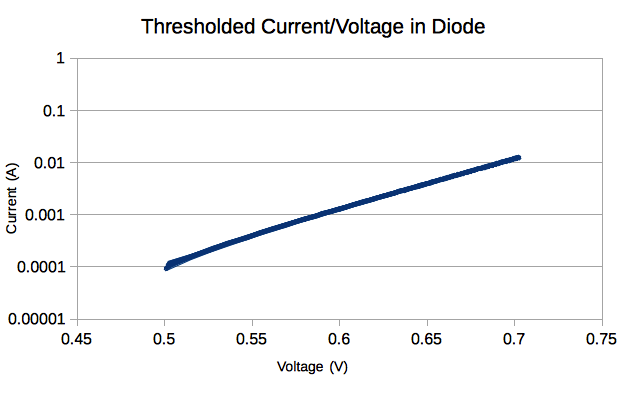
\includegraphics[width=70mm]{dio_thresh.png}
\caption{Thresholded log plot of current in a forward-driven diode.}
\label{fig:dio_thresh}
\end{figure}

The RC curve demonstrates the transient behavior of a capacitor - upon voltage
being applied, it gradually collects charge, with the voltage across it
increasing until it is equal to the total voltage across the circuit. The curve
itself is an exponential that approaches the target voltage, and like any
exponential has a characteristic time constant that describes it.

\begin{displaymath}
V = V_b \left(1 - e^{-\frac{t}{RC}}\right)
\end{displaymath} 

In this case, the time constant $\tau = RC$ is the amount of time it takes for
the difference between the capacitor voltage and circuit voltage to fall by a
factor of e. This constant can be found by manipulating the equation and taking
the logarithm of both sides, yielding Equation~\ref{rc_logarithm}.

\begin{equation}
\label{rc_logarithm}
ln(V_b - V) = ln(V_b) - \frac{t}{RC}
\end{equation}

Figure~\ref{fig:rc_response} has several potential regions that could be used
for this analysis - the portion used is shown in Figure~\ref{fig:rc_linear}.

\begin{figure}[ht!]
\centering
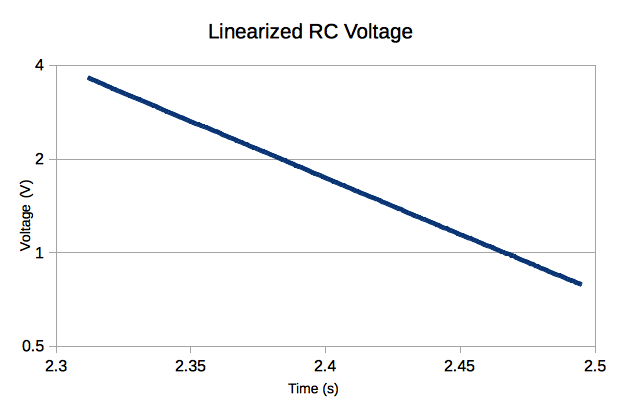
\includegraphics[width=70mm]{rc_linear.png}
\caption{Log plot of capacitor charging under a constant voltage.}
\label{fig:rc_linear}
\end{figure}

A linear regression returns a slope of m = \mval{8.369}{0.003}{}. This slope is
equal to the negative inverse time constant in Equation~\ref{rc_logarithm}.
This means the time constant itself is

\begin{displaymath}
\tau = RC = -\frac{1}{m}
\end{displaymath} 

With an uncertainty of

\begin{displaymath}
\sigma _{\bar \tau} = \frac{\sigma _{\bar m}}{\bar m^2}
\end{displaymath} 

Which yields RC = \mval{0.11949}{0.00004}{s}. This is remarkably close to the
predicted value of \mval{0.1195}{0.00005}{s}. 

The RLC circuit had a relatively clear resonance at \mval{530}{50}{Hz}. The
uncertainty is based on the width of the region of the peak with
nearly-identical amplitude. The theoretical value could be predicted using
Equation~\ref{resonant_freq}.

\begin{equation}
\label{resonant_freq}
f_{res} = \frac{1}{2 \pi \sqrt{LC}}
\end{equation}

Using the values of the inductor and capacitor, the predicted frequency is 503
Hz, which is only a 5.3\% difference. This could be explained by the relatively
high uncertainty in the resonance peak - it was not large enough to get a clear
reading, and the theoretical value falls within its range.

The curve also does not the range necessary to find the Q-factor of this
circuit. It only holds the top of the peak, and does not get close to
$1/\sqrt{2}$ of the peak voltage. However, it does follow Equation~\ref{v_out}

\begin{equation}
\label{v_out}
V = \frac{V_{in}}{\sqrt{R^2 + \left(\omega L - \frac{1}{\omega C} \right)^2}}
\end{equation}

A linear regression was performed to find the right coefficients, and these
could be used to extrapolate the points at which the amplitude is $1/\sqrt{2}$
of the peak - \mval{18.9}{0.2}{Hz} and \mval{15520}{60}{Hz}. Using these, the Q
factor is easy to find using Equation~\ref{Q_fact}

\begin{equation}
\label{Q_fact}
Q = \frac{f_{res}}{f_2 - f_1}
\end{equation}

The Q factor is \mval{28}{3}{}.

\section{Conclusion}

The results of experiment and theoretical calculations ended up being
remarkably close. The largest differences took place in the RLC circuit and the
diode response curve. The former makes sense - there was a large uncertainty
caused by a bad choice of circuit elements (100 mH is too large for a narrow
peak). However, even with a 5.3\% difference, the theoretical frequency fell
within the uncertainty of the calculated value. Using a different inductor
would likely fix the issue in a future experiment.

The diode calculations, on the other hand, resulted in a much larger difference
for $e/k_B$, but for a similarly simple reason. The calculated value was based
    on invalid assumptions about the constants to do with the circuit, and
    these assumptions did not include the uncertainty. The n factor for a diode
    can vary from 1 to 2, however, and the value was off by only 15.3\% (11000
    vs 13000) - it is likely that the systematic uncertainty came from the
    assumptions about the value of n and not a flaw in the exponential model.

The other calculations, of the resistor value and RC time constant, were
remarkably close. The former was measured at 993, versus a calculated value of
992.5, and the latter was predicted to be 0.1195 seconds, versus a calculated
0.11949. These agree perfectly to within the uncertainties used.

\end{document}


